\documentclass[12pt,letterpaper]{article}
\usepackage{graphicx,textcomp}
\usepackage{natbib}
\usepackage{setspace}
\usepackage{fullpage}
\usepackage{color}
\usepackage[reqno]{amsmath}
\usepackage{amsthm}
\usepackage{fancyvrb}
\usepackage{amssymb,enumerate}
\usepackage[all]{xy}
\usepackage{endnotes}
\usepackage{lscape}
\newtheorem{com}{Comment}
\usepackage{float}
\usepackage{hyperref}
\newtheorem{lem} {Lemma}
\newtheorem{prop}{Proposition}
\newtheorem{thm}{Theorem}
\newtheorem{defn}{Definition}
\newtheorem{cor}{Corollary}
\newtheorem{obs}{Observation}
\usepackage[compact]{titlesec}
\usepackage{dcolumn}
\usepackage{tikz}
\usetikzlibrary{arrows}
\usepackage{multirow}
\usepackage{xcolor}
\newcolumntype{.}{D{.}{.}{-1}}
\newcolumntype{d}[1]{D{.}{.}{#1}}
\definecolor{light-gray}{gray}{0.65}
\usepackage{url}
\usepackage{listings}
\usepackage{color}

\definecolor{codegreen}{rgb}{0,0.6,0}
\definecolor{codegray}{rgb}{0.5,0.5,0.5}
\definecolor{codepurple}{rgb}{0.58,0,0.82}
\definecolor{backcolour}{rgb}{0.95,0.95,0.92}

\lstdefinestyle{mystyle}{
	backgroundcolor=\color{backcolour},   
	commentstyle=\color{codegreen},
	keywordstyle=\color{magenta},
	numberstyle=\tiny\color{codegray},
	stringstyle=\color{codepurple},
	basicstyle=\footnotesize,
	breakatwhitespace=false,         
	breaklines=true,                 
	captionpos=b,                    
	keepspaces=true,                 
	numbers=left,                    
	numbersep=5pt,                  
	showspaces=false,                
	showstringspaces=false,
	showtabs=false,                  
	tabsize=2
}
\lstset{style=mystyle}
\newcommand{\Sref}[1]{Section~\ref{#1}}
\newtheorem{hyp}{Hypothesis}

\title{Problem Set 2}
\date{Due: October 23, 2025}
\author{Applied Stats/Quant Methods 1}

\begin{document}
	\maketitle
	\section*{Instructions}
\begin{itemize}
	\item Please show your work! You may lose points by simply writing in the answer. If the problem requires you to execute commands in \texttt{R}, please include the code you used to get your answers. Please also include the \texttt{.R} file that contains your code. If you are not sure if work needs to be shown for a particular problem, please ask.
	\item Your homework should be submitted electronically on GitHub.
	\item This problem set is due before 23:59 on Thursday October 23, 2025. No late assignments will be accepted.

\end{itemize}

	
	\vspace{.5cm}
	\section*{Question 1: Political Science}
		\vspace{.25cm}
	The following table was created using the data from a study run in a major Latin American city.\footnote{Fried, Lagunes, and Venkataramani (2010). ``Corruption and Inequality at the Crossroad: A Multimethod Study of Bribery and Discrimination in Latin America. \textit{Latin American Research Review}. 45 (1): 76-97.} As part of the experimental treatment in the study, one employee of the research team was chosen to make illegal left turns across traffic to draw the attention of the police officers on shift. Two employee drivers were upper class, two were lower class drivers, and the identity of the driver was randomly assigned per encounter. The researchers were interested in whether officers were more or less likely to solicit a bribe from drivers depending on their class (officers use phrases like, ``We can solve this the easy way'' to draw a bribe). The table below shows the resulting data.

\newpage
\begin{table}[h!]
	\centering
	\begin{tabular}{l | c c c }
		& Not Stopped & Bribe requested & Stopped/given warning \\
		\\[-1.8ex] 
		\hline \\[-1.8ex]
		Upper class & 14 & 6 & 7 \\
		Lower class & 7 & 7 & 1 \\
		\hline
	\end{tabular}
\end{table}

\begin{enumerate}
	
	\item [(a)]
	Calculate the $\chi^2$ test statistic by hand/manually (even better if you can do "by hand" in \texttt{R}).\\
	
	I will calculate the $\chi^2$ test statistic by hand to determine whether the difference between both categorical variables is statistically significant.
	
	I will do it in R and the first step will be creating the table there.
	
	\lstinputlisting[language=R, firstline=1, lastline=20]{PS2_answers_RLP.R} 
	
	The  $\chi^2$ test statistic of these categorical variables has a value of 3.7912.
	
	\vspace{1cm}
	\item [(b)]
	Now calculate the p-value from the test statistic you just created (in \texttt{R}).\footnote{Remember frequency should be $>$ 5 for all cells, but let's calculate the p-value here anyway.}  What do you conclude if $\alpha = 0.1$?\\
	
		\lstinputlisting[language=R, firstline=22, lastline=34]{PS2_answers_RLP.R} 
	
	As I can't reject the null hypothesis, I can't affirm that the officers are more or less likely to solicit a bribe from drivers based on their social class.
	
	\newpage
	\item [(c)] Calculate the standardized residuals for each cell and put them in the table below.
	\vspace{1cm}
	
	\lstinputlisting[language=R, firstline=36, lastline=45]{PS2_answers_RLP.R} 
	
	\begin{table}[h]
		\centering
		\begin{tabular}{l | c c c }
			& Not Stopped & Bribe requested & Stopped/given warning \\
			\\[-1.8ex] 
			\hline \\[-1.8ex]
			Upper class  &0.32  &-1.64  &1.52  \\
			\\
			Lower class &-0.32  &1.64   &-1.52   \\
			
		\end{tabular}
	\end{table}
	
	
	\vspace{1cm}
	\item [(d)] How might the standardized residuals help you interpret the results? 
	
	As any of these standardized residual values is over 2 or below -2, there is no strong evidence of association between both variables (class and police officer treatment).
	
\end{enumerate}
\newpage

\section*{Question 2: Economics}
Chattopadhyay and Duflo were interested in whether women promote different policies than men.\footnote{Chattopadhyay and Duflo. (2004). ``Women as Policy Makers: Evidence from a Randomized Policy Experiment in India. \textit{Econometrica}. 72 (5), 1409-1443.} Answering this question with observational data is pretty difficult due to potential confounding problems (e.g. the districts that choose female politicians are likely to systematically differ in other aspects too). Hence, they exploit a randomized policy experiment in India, where since the mid-1990s, $\frac{1}{3}$ of village council heads have been randomly reserved for women. A subset of the data from West Bengal can be found at the following link: \url{https://raw.githubusercontent.com/kosukeimai/qss/master/PREDICTION/women.csv}\\

\noindent Each observation in the data set represents a village and there are two villages associated with one GP (i.e. a level of government is called "GP"). Figure~\ref{fig:women_desc} below shows the names and descriptions of the variables in the dataset. The authors hypothesize that female politicians are more likely to support policies female voters want. Researchers found that more women complain about the quality of drinking water than men. You need to estimate the effect of the reservation policy on the number of new or repaired drinking water facilities in the villages.
\vspace{.5cm}
\begin{figure}[h!]
	\caption{\footnotesize{Names and description of variables from Chattopadhyay and Duflo (2004).}}
	\vspace{.5cm}
	\centering
	\label{fig:women_desc}
	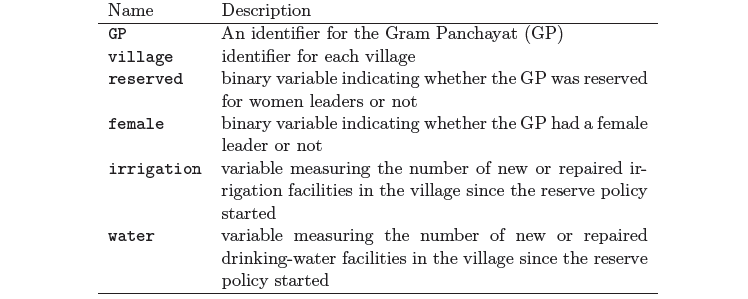
\includegraphics[width=1.1\textwidth]{"C:/Users/Usuario/Documents/GitHub/StatsI_2025/problemSets/PS02/template/women_desc.png"}
\end{figure}		

\newpage
\begin{enumerate}
	\item [(a)] State a null and alternative (two-tailed) hypothesis.
	\vspace{1cm}
	
	A two-tailed hypothesis posits that there is a significant difference or relationship between two groups or variables without specifying the direction of the difference. Therefore, following Chattopadhyay and Duflo (2004), I will hypothesise (H{1}) that the amount of new or repaired drinking-water facilities in the village is different when between female- and male-led Gram Panchayats. However, I will not specify--in my hypothesis--whether the amount will be bigger or smaller in each case. By the same token, the null hypothesis (H{0}) will suggest that there is no difference.
	
	\vspace{1cm}
	
	H{0}: there is no difference in the number of new or repaired drinking-water facilities between female- and male-led Gram Panchayats.
	


	H{1}: there is a difference in the number of new or repaired drinking-water facilities between female- and male-led Gram Panchayats.
	
	\vspace{2cm}
	\item [(b)] Run a bivariate regression to test this hypothesis in \texttt{R} (include your code!).
	
	\lstinputlisting[language=R, firstline=51, lastline=56]{PS2_answers_RLP.R} 
	
	\begin{figure}[h]
		\centering
		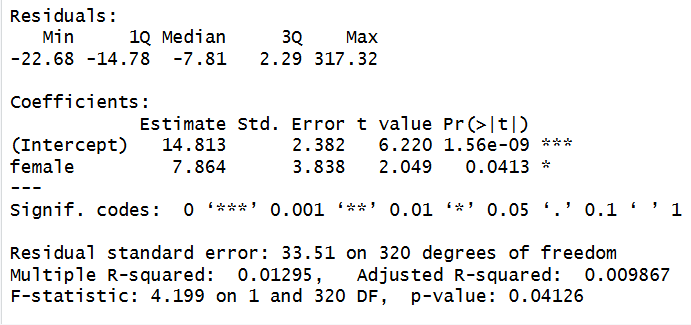
\includegraphics[width=0.75\linewidth]{regression_output1.png}
	\end{figure}
	
	The coefficient for female is positive (7.86) and statistically significant (p = 0.041), indicating that Gram Panchayats headed by women have, on average, built 7.86 more drinking-water facilities than those headed by men. This result supports hypothesis (H{1}) that the amount of new or repaired drinking-water facilities in the village is different when between female- and male-led Gram Panchayats. As we can identify a statistically significant difference in the number of drinking-water facilities between male- and female-headed Gram Panchayats, we can reject the null hypothesis (H{0}).
	

	
	
	\vspace{1cm}
	\item [(c)] Interpret the coefficient estimate for reservation policy. 
	
		\lstinputlisting[language=R, firstline=58, lastline=61]{PS2_answers_RLP.R} 
	
	\begin{figure}[h]
		\centering
		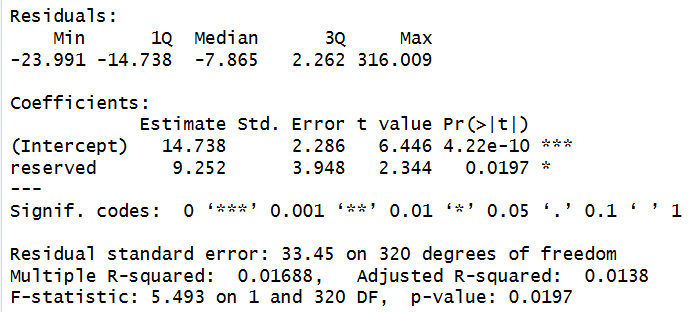
\includegraphics[width=0.75\linewidth]{regression_output2.png}
	\end{figure}
	
		The coefficient for reservation policy is positive (9.252) and statistically significant (p = 0.0197), indicating that Gram Panchayats affected by the reservation policy have, on average, built 9.252 more drinking-water facilities than those that were not affected by the policy.
	
\end{enumerate}


%\end{enumerate}
\end{document}
